% -*- coding: utf-8; -*-
% vim: set fileencoding=utf-8 :

% The paper on using Luau telemetry to measure the effectiveness of type error reporting.

\documentclass[english,submission,cleveref]{programming}
%% use 'submission' for initial submission, remove it for camera-ready (see 5.1)

%%\overfullrule=1mm

%% BEGIN tobias pape 2021-11-06
% Why do we need this? To have headings in the abstract.
\makeatletter
\newcommand*\abstractpart[1]{\unskip\par\noindent{\firamedium\color{P@GrayFG}{#1}}\enspace}
\makeatother
%% END

\usepackage{alltt}
% Not sure why <Programming> is recommending non-standard tools
% \usepackage[backend=biber]{biblatex}
\usepackage{amssymb}
\usepackage{calc}
\usepackage{colortbl}
\usepackage{listings}
\usepackage{mathpartir}
\usepackage{pifont}
% Errors with
% ! Undefined control sequence.
% <argument> \l__siunitx_number_implicit_plus_bool 
% l.61 \begin{document}
% using Mac TeXlive 20230313_2
% \usepackage{siunitx}
\usepackage{tikz}
\usepackage{subcaption}
\usepackage{wasysym}
\usepackage{xcolor}
\usetikzlibrary{shapes.geometric}

%%%%%%%%%%%%%%%%%%
\paperdetails{
  %% perspective options are: art, sciencetheoretical, scienceempirical, engineering.
  %% Choose exactly the one that best describes this work. (see 2.1)
  perspective=scienceempirical,
  %% State one or more areas, separated by a comma. (see 2.2)
  %% Please see list of areas in http://programming-journal.org/cfp/
  %% The list is open-ended, so use other areas if yours is/are not listed.
  area={Data mining for programming, Telemetry},
  %% You may choose the license for your paper (see 3.)
  %% License options include: cc-by (default), cc-by-nc
  % license=cc-by,
}
%%%%%%%%%%%%%%%%%%

%%%%%%%%%%%%%%%%%%
%% These data are provided by the editors. May be left out on submission.
%\paperdetails{
%  submitted=2023-1-31,
%  published=2016-10-11,
%  year=2016,
%  volume=1,
%  issue=1,
%  articlenumber=1,
%}
%%%%%%%%%%%%%%%%%%

\begin{document}

\title{Type Error Telemetry at Scale: Pseudonymized and Stochiastic}
% lean, lite, modest, non-intrusive, private, ...
% {Millions of Type Errors} = 72M forced strict, 1/2M type error is disappointing!
%% \subtitle{Impersonal Telemetry to Measure User Experience}

% Alphabetical order for authors?

\author[a]{Ben Greenman}
\authorinfo{(\email{benjamin.l.greenman@gmail.com}) is a postdoc at Brown University. He will be joining the University of Utah in Fall~2023.}
\affiliation[a]{Brown University, Providence, RI, USA}
% \orcid{0000-0001-7078-9287}

\author[b]{Alan Jeffrey}
\authorinfo{(\email{ajeffrey@roblox.com}) is a Principal Software Engineer at Roblox.}
% \orcid{0000-0001-6342-0318}
\affiliation[b]{Roblox, San Mateo, CA, USA}

\author[a]{Shriram Krishnamurthi}
% \orcid{0000-0001-5184-1975}
\authorinfo{(\email{shriram@brown.edu}) is the Vice President of Programming Languages (no, not really) at Brown University.}

\author[b]{Mitesh Shah}
\authorinfo{(\email{mshah@roblox.com}) is Senior Engineering Director, Programmability, at Roblox.}

%\renewcommand{\shortauthors}{...}

\newcommand{\code}[1]{\texttt{#1}}
\newcommand{\FILL}{\textbf{FILL}}
\newcommand{\dotscale}[1]{\scalebox{0.72}{#1}}
\newcommand{\wideas}[2]{\makebox[\widthof{#2}][l]{#1}}
\newcommand{\twoline}[2]{\parbox[s]{1.4cm}{\flushleft#1\newline#2}}
\newcommand{\chkYes}{\dotscale{\CIRCLE}}
\newcommand{\chkMaybe}{\wideas{\dotscale{\Circle}}{\chkYes}}
\newcommand{\chkNo}{\wideas{}{\chkYes}}
\newcommand{\pct}[1]{\SI{#1}{\percent}}
\newcommand{\modefont}[1]{\texttt{#1}}
\newcommand{\mnocheck}{\modefont{nocheck}}
\newcommand{\mnonstrict}{\modefont{nonstrict}}
\newcommand{\mstrict}{\modefont{strict}}
\newcommand{\zerowidth}[1]{\makebox[0pt][l]{#1}}
\newcommand{\stddev}[1]{[#1\textsc{k}]}
\newcommand{\gcell}[1]{\cellcolor{green!20}#1}
\newcommand{\ycell}[1]{\cellcolor{yellow!18}#1}
\newcommand{\ocell}[1]{\cellcolor{orange!29}#1}
\newcommand{\rcell}[1]{\cellcolor{red!30}$\!\!$#1$\!\!$}
\newcommand{\gbox}[1]{\colorbox{green!20}{#1}}
\newcommand{\ybox}[1]{\colorbox{yellow!18}{#1\vphantom{Ap}}}
\newcommand{\obox}[1]{\colorbox{orange!29}{#1\vphantom{Ap}}}
\newcommand{\rbox}[1]{\colorbox{red!30}{#1\vphantom{Ap}}}

%%
%% The code below is generated by the tool at http://dl.acm.org/ccs.cfm.
%% Please copy and paste the code instead of the example below.

\begin{CCSXML}
<ccs2012>
<concept>
<concept_id>10002944.10011123.10010916</concept_id>
<concept_desc>General and reference~Measurement</concept_desc>
<concept_significance>500</concept_significance>
</concept>
</ccs2012>
\end{CCSXML}

\ccsdesc[500]{General and reference~Measurement}

\keywords{types, gradual typing, telemetry, user study, large-scale study}

\maketitle

\begin{abstract}
  \let\paragraph\abstractpart

  \paragraph{Context}
  %% What is the broad context of the work? What is
  %% the importance of the general research area?
  {Roblox Studio} lets millions of creators
  build interactive experiences by programming in a variant
  of Lua called Luau.
  The creators form a broad group, ranging from novices writing
  their first script to professional developers, thus Luau
  must support a wide audience.
  As part of its efforts to support all kinds programmers, Luau includes a
  gradual type system and goes to great lengths to minimize false positive
  errors.

  \paragraph{Inquiry}
  %% What problem or question does the paper
  %% address? How has this problem or question been
  %% addressed by others (if at all)?
  Since Luau is in the hands of many creators, we want to collect their feedback
  and ultimately improve the language design (in particular, the type system).
  We want feedback at a large scale, as creators work on their actual projects,
  which suggests the deployment of client-side telemetry.
  %% ^ awkward
  However, we must respect creators privacy.
  Whatever telemetry we use to study the Luau language cannot include
  personally-identifiable information.
  For example, we cannot monitor source code or error messages as they
  may contain personal data.
  Finding ways to harness telemetry in a private way is the central research challenge.

  \paragraph{Approach}
  %% What was done that unveiled new knowledge?
  We designed and implemented a privacy-preserving telemetry system for Luau.
  Telemetry records include a timestamp, a (randomized) session id, a reason
  for sending, and a sequence of counter values summarizing the results of type
  analysis.
  Over four months in Spring 2023, we deployed the telemetry system and collected
  1.5 million telemetry records.
  We analyzed the data to improve Luau.

  \paragraph{Knowledge}
  %% What new facts were uncovered? If the
  %% research was not results oriented, what new
  %% capabilities are enabled by the work?
  We present several findings about Luau:
  some confirm hypotheses by the Luau team, others are rather surprising, but
  all findings support our claim that privacy-preserving telemetry is a useful
  way to collect feedback.
  One expected finding is that types are unpopular; there is an order-of-maginitude
  difference in the number of sessions that use different type analysis modes.
  One surprise is that the strict type analysis mode evidently makes it difficult
  to connect a script with data assets.
  Lastly, one reassuring finding is that type analysis rarely hits its internal
  limits on problem size.

  \paragraph{Grounding}
  %% What argument, feasibility proof, artifacts,
  %% or results and evaluation support this work?
  Our findings are supported by a publicly-available dataset
  of over 1.5 million telemetry records
  and by free software for analyzing the data.

  \paragraph{Importance}
  %% Why does this work matter?
  Luau is the first large-scale combination of gradual types and semantic
  subtyping.
  Beyond the immediate benefits to Luau,
  our findings about types and type errors have implications
  for adoption and ergonomics in other gradual languages.
  %% mention Elixir, Verse?
  FILL specifics.
  Our telemetry design is of broad interest, as it gathers useful
  data without exposing personal information.

\end{abstract}

\section{Introduction}
\label{s:introduction}

{Roblox} is a platform for {shared virtual experiences}, with
65~million Daily Active Users, and 14~billion hours of engagement in
April--June 2023; there are 3~million creators using {Roblox Studio},
creating 5~million experiences~\cite{corp.roblox.com}.

{Roblox experiences} are scripted using the 
{Luau} programming language~\cite{luau-lang.org},
an extension of {Lua~5.1~\cite{lua}}.
The main extension is the addition of a static type system, which uses
type inference to synthesize types for user code on the fly.
These types are used primarily in type-driven tooling such as autocomplete and
API documentation~\cite{luau-autocomplete}, but creators can also opt in to
receiving type error reports.

As discussed in~\cite{bfj-hatra-2021},
the goals of the {Luau} type system are rather different from
a traditional type system, which focuses on compilation and memory safety.
{Luau} has a diverse user community, ranging from
students in code camps to professional development studios. These
creators have quite different needs, with different emphases on
enabling rapid creation and ensuring software quality.
{Luau} therefore supports three typing modes---\mstrict{} types,
relaxed (\mnonstrict{}) types, and no types (\mnocheck{})---and lets users switch
between modes gradually~\cite{st-sfp-2006,tfffgksst-snapl-2017}, one module at a time.

In this paper, we investigate methods for measuring the effectiveness
of the {Luau} type system in the development of {Roblox} scripts.
We want to collect measurements at a large scale, with thousands
of participants, and we must do so in a way that protects creators' privacy.
In comparison to prior work~(\cref{s:related}), which
with few exceptions~\cite{zhlbr-cc-2020,zhlbr-oopsla-2020,hlzbr-ecoop-2021} is either small in scale
or collects personally identifiable information~(PII),
we performed a large-scale study using pseudonymized \emph{telemetry}.

{Roblox Studio} has a telemetry system, which is used to gauge
the effectiveness of creation features. This system stochastically
determines which sessions should report telemetry, and for those
sessions, reports telemetry records back with a summary of the
session. In the case of this study, the telemetry includes data on the
number of errors at various levels of granularity: in the current edit
range, in the current file, and in every file which was type
checked.

The telemetry data we analyzed does not contain any PII.
It has no source code;
 no source locations;
no error messages (which may contain source code);
no error messages;
no record of the creator's identity, locale, or IP address;
and no information about what creation the data came from.
Telemetry records are correlated by session, using a pseudonymized
session identifier.

Most users of {Roblox Studio} do not opt in to type error
reporting, and so they do not see the ``squiggly underlining'' that
indicates a type error site. Nonetheless, the type inference system
still runs in the background (since it drives autocomplete and other
type-based tools), letting us see which type errors would have
been reported and whether users fix these errors over time.

With this telemetry data, we investigate research questions about
the adoption and benefits of type analysis:
\begin{description}
  \item[RQ1.]
    How many creators use type analysis?
    How often do projects contain modules with different
    analysis modes?
    How often do creators turn analysis off?
  \item[RQ2.]
    For modules that use type analysis:
    which errors arise,
    how do creators respond,
    and which errors tend to persist despite subsequent edits?
  \item[RQ3.]
    What impact does type analysis have on the number of background type
    errors?
    For example, do background errors pile up in unanalyzed projects?
\end{description}

Beyond their immediate applications to {Luau},
answers to these questions have implications for the design
of gradual types~\cite{st-sfp-2006}, success types~\cite{lindahl2006practical},
and semantic subtyping~\cite{CF05:GentleIntroduction,Jef22:SemanticSubtyping}.
Luau represents the first large-scale combination of these features,
and lessons from this experience can inform future applications.

At a higher level, this paper is the first to use telemetry 
to study a typechecker.
It thus represents a step toward data-driven language design,
informed by many users' actual practice.
Our data captures over 340,000 sessions
that occured between February and April 2023
and includes 72 million type analysis errors.
By contrast to typical qualitative methods (e.g., surveys and interviews), it
is not restricted to users' \emph{perceptions} about their work and it is not
limited to a small number of users.

FILL can stats answer questions that point-by-point analysis cannot?

\paragraph{Contributions}
\begin{itemize}
  \item
    Design of a low-overhead, (black-box / PII-safe / impersonal)
    telemetry method, that other
    researchers can build on.

  \item
    Lessons from millions of type errors about
    the adoption of strict type analysis,
    the usefulness of type errors,
    and \FILL{}.
    These findings are especially important for the
    gradual typing, success typing, and semantic subtyping communities.

  \item
    \FILL{} any surprises when doing the analysis?
    Note, no ML for analysis, we do not have a corpus of text.

\end{itemize}

Analysis pipeline to be freely available.
Data may be available, depends on Roblox.


\section{{Roblox} Context}
% https://create.roblox.com/docs/scripting/luau

FILL table = object

\begin{figure}

  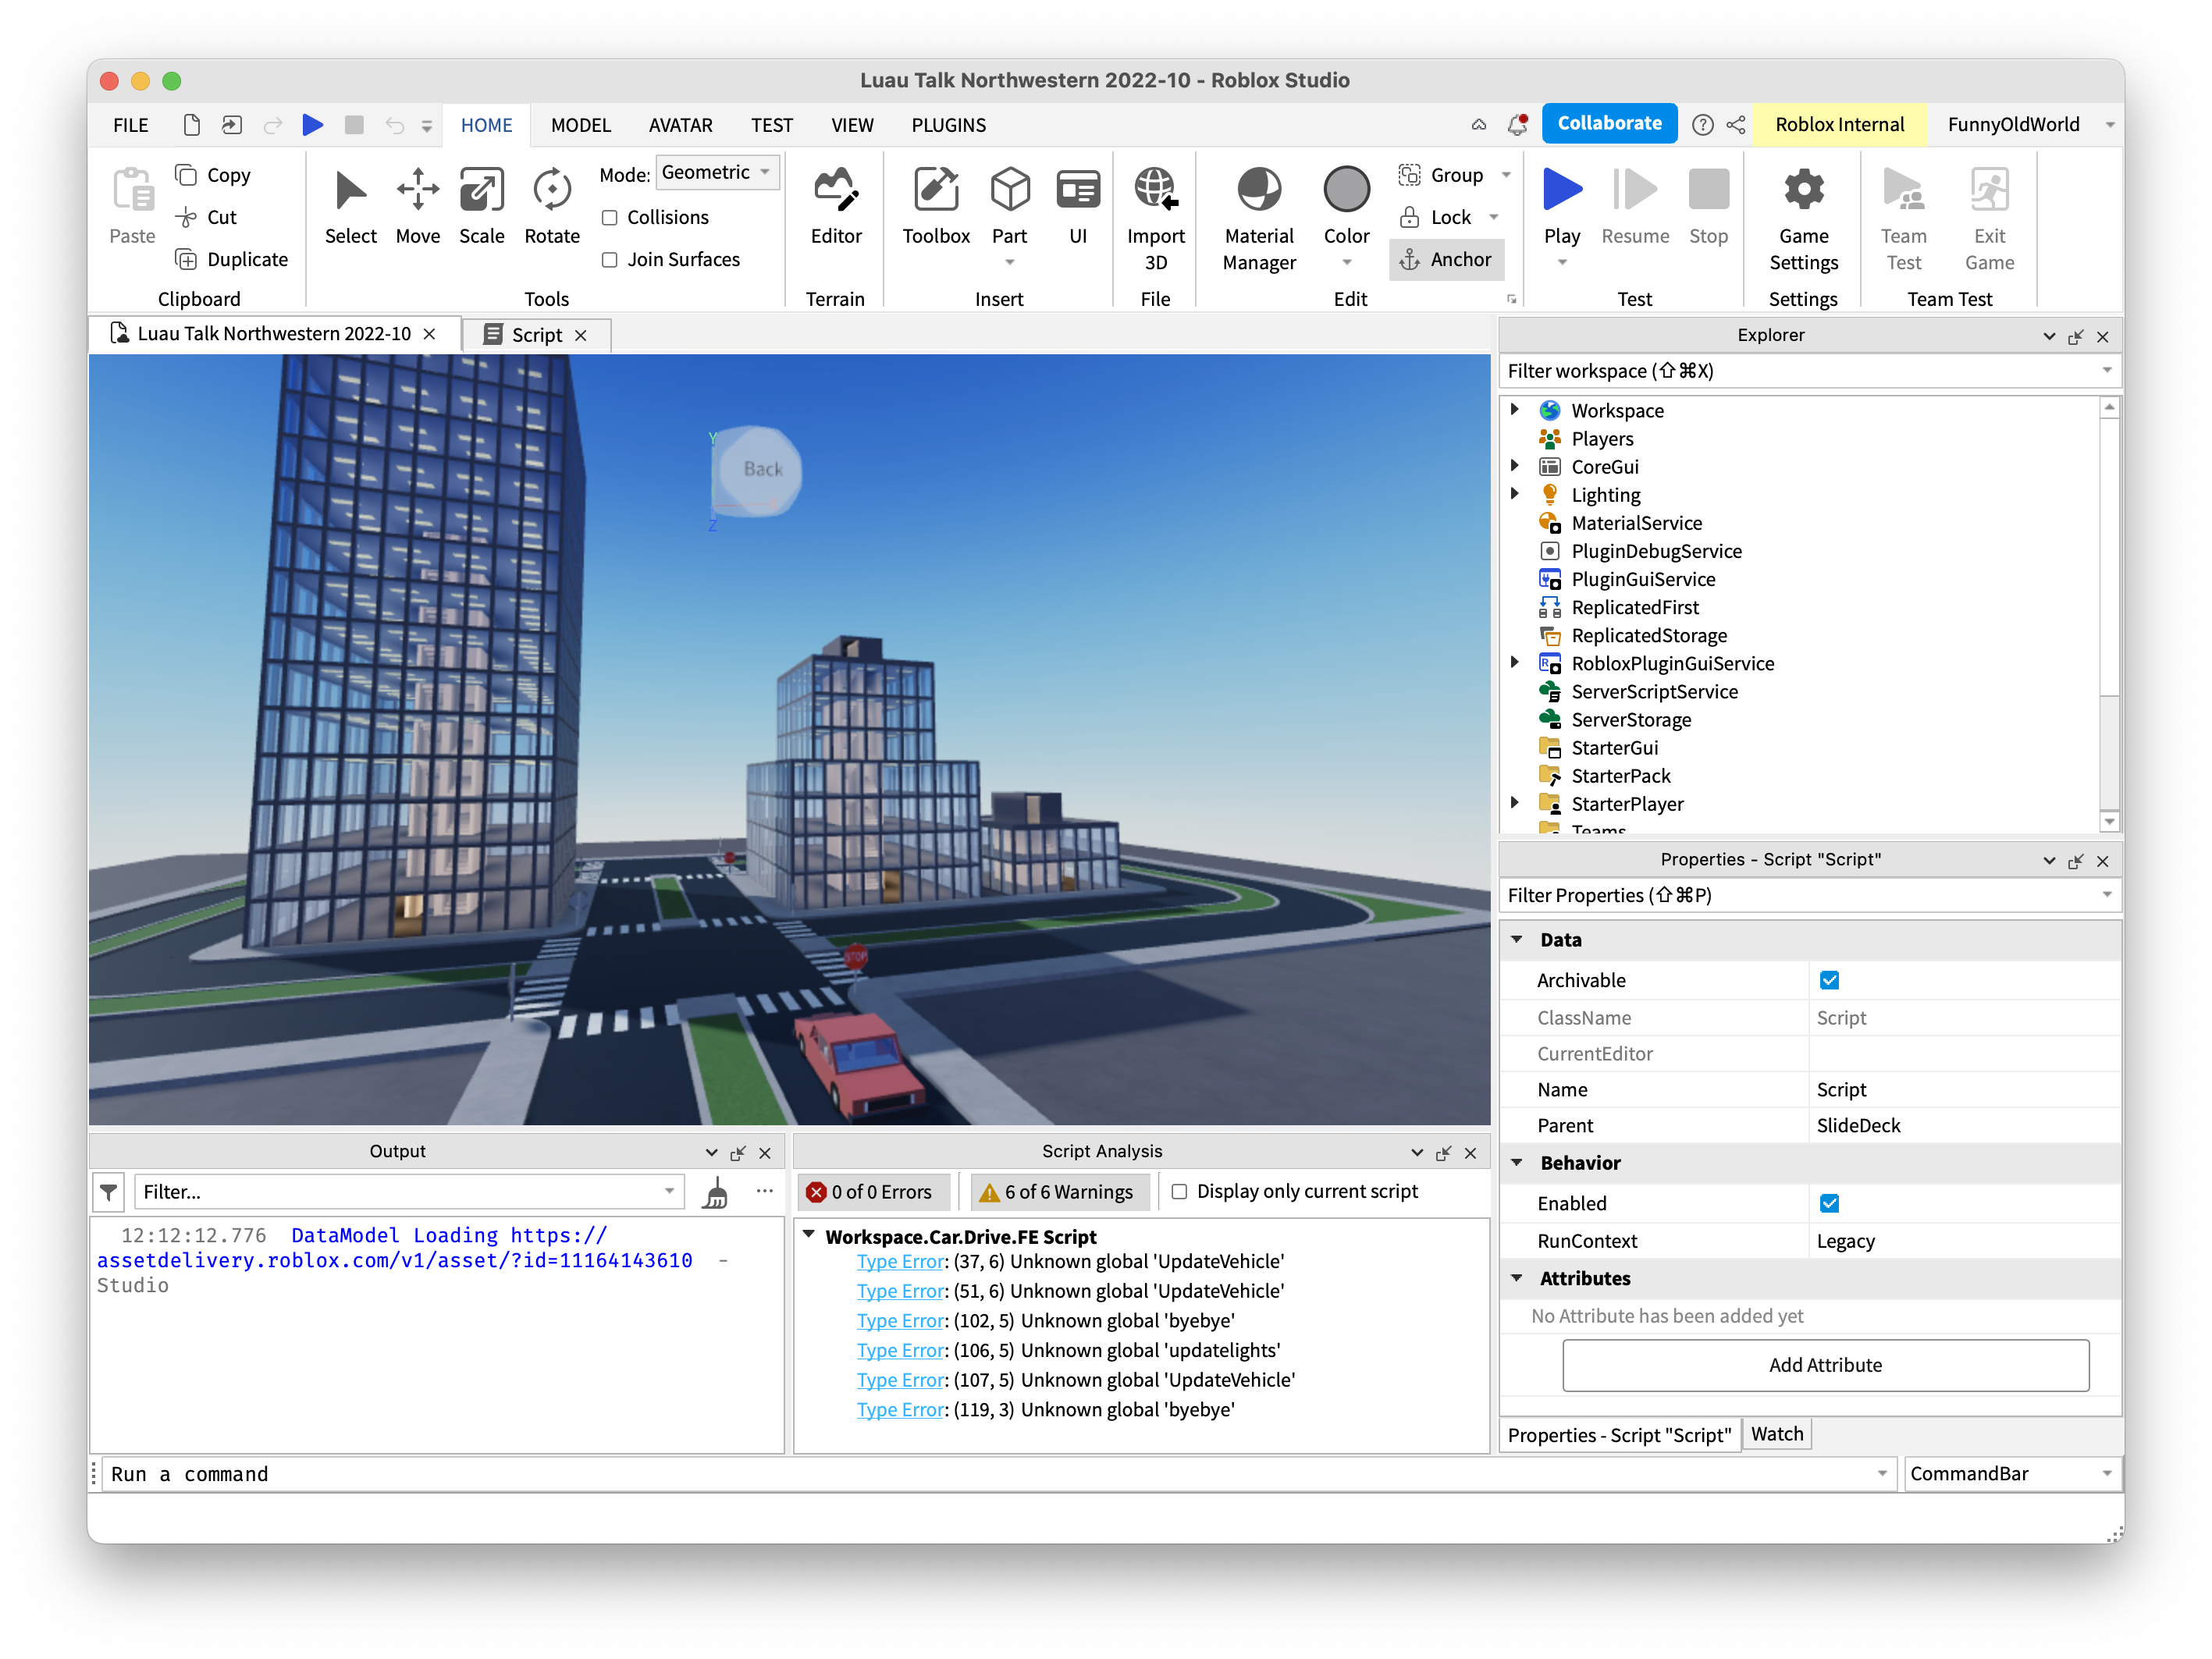
\includegraphics[width=.45\textwidth]{img/roblox-studio.png}
  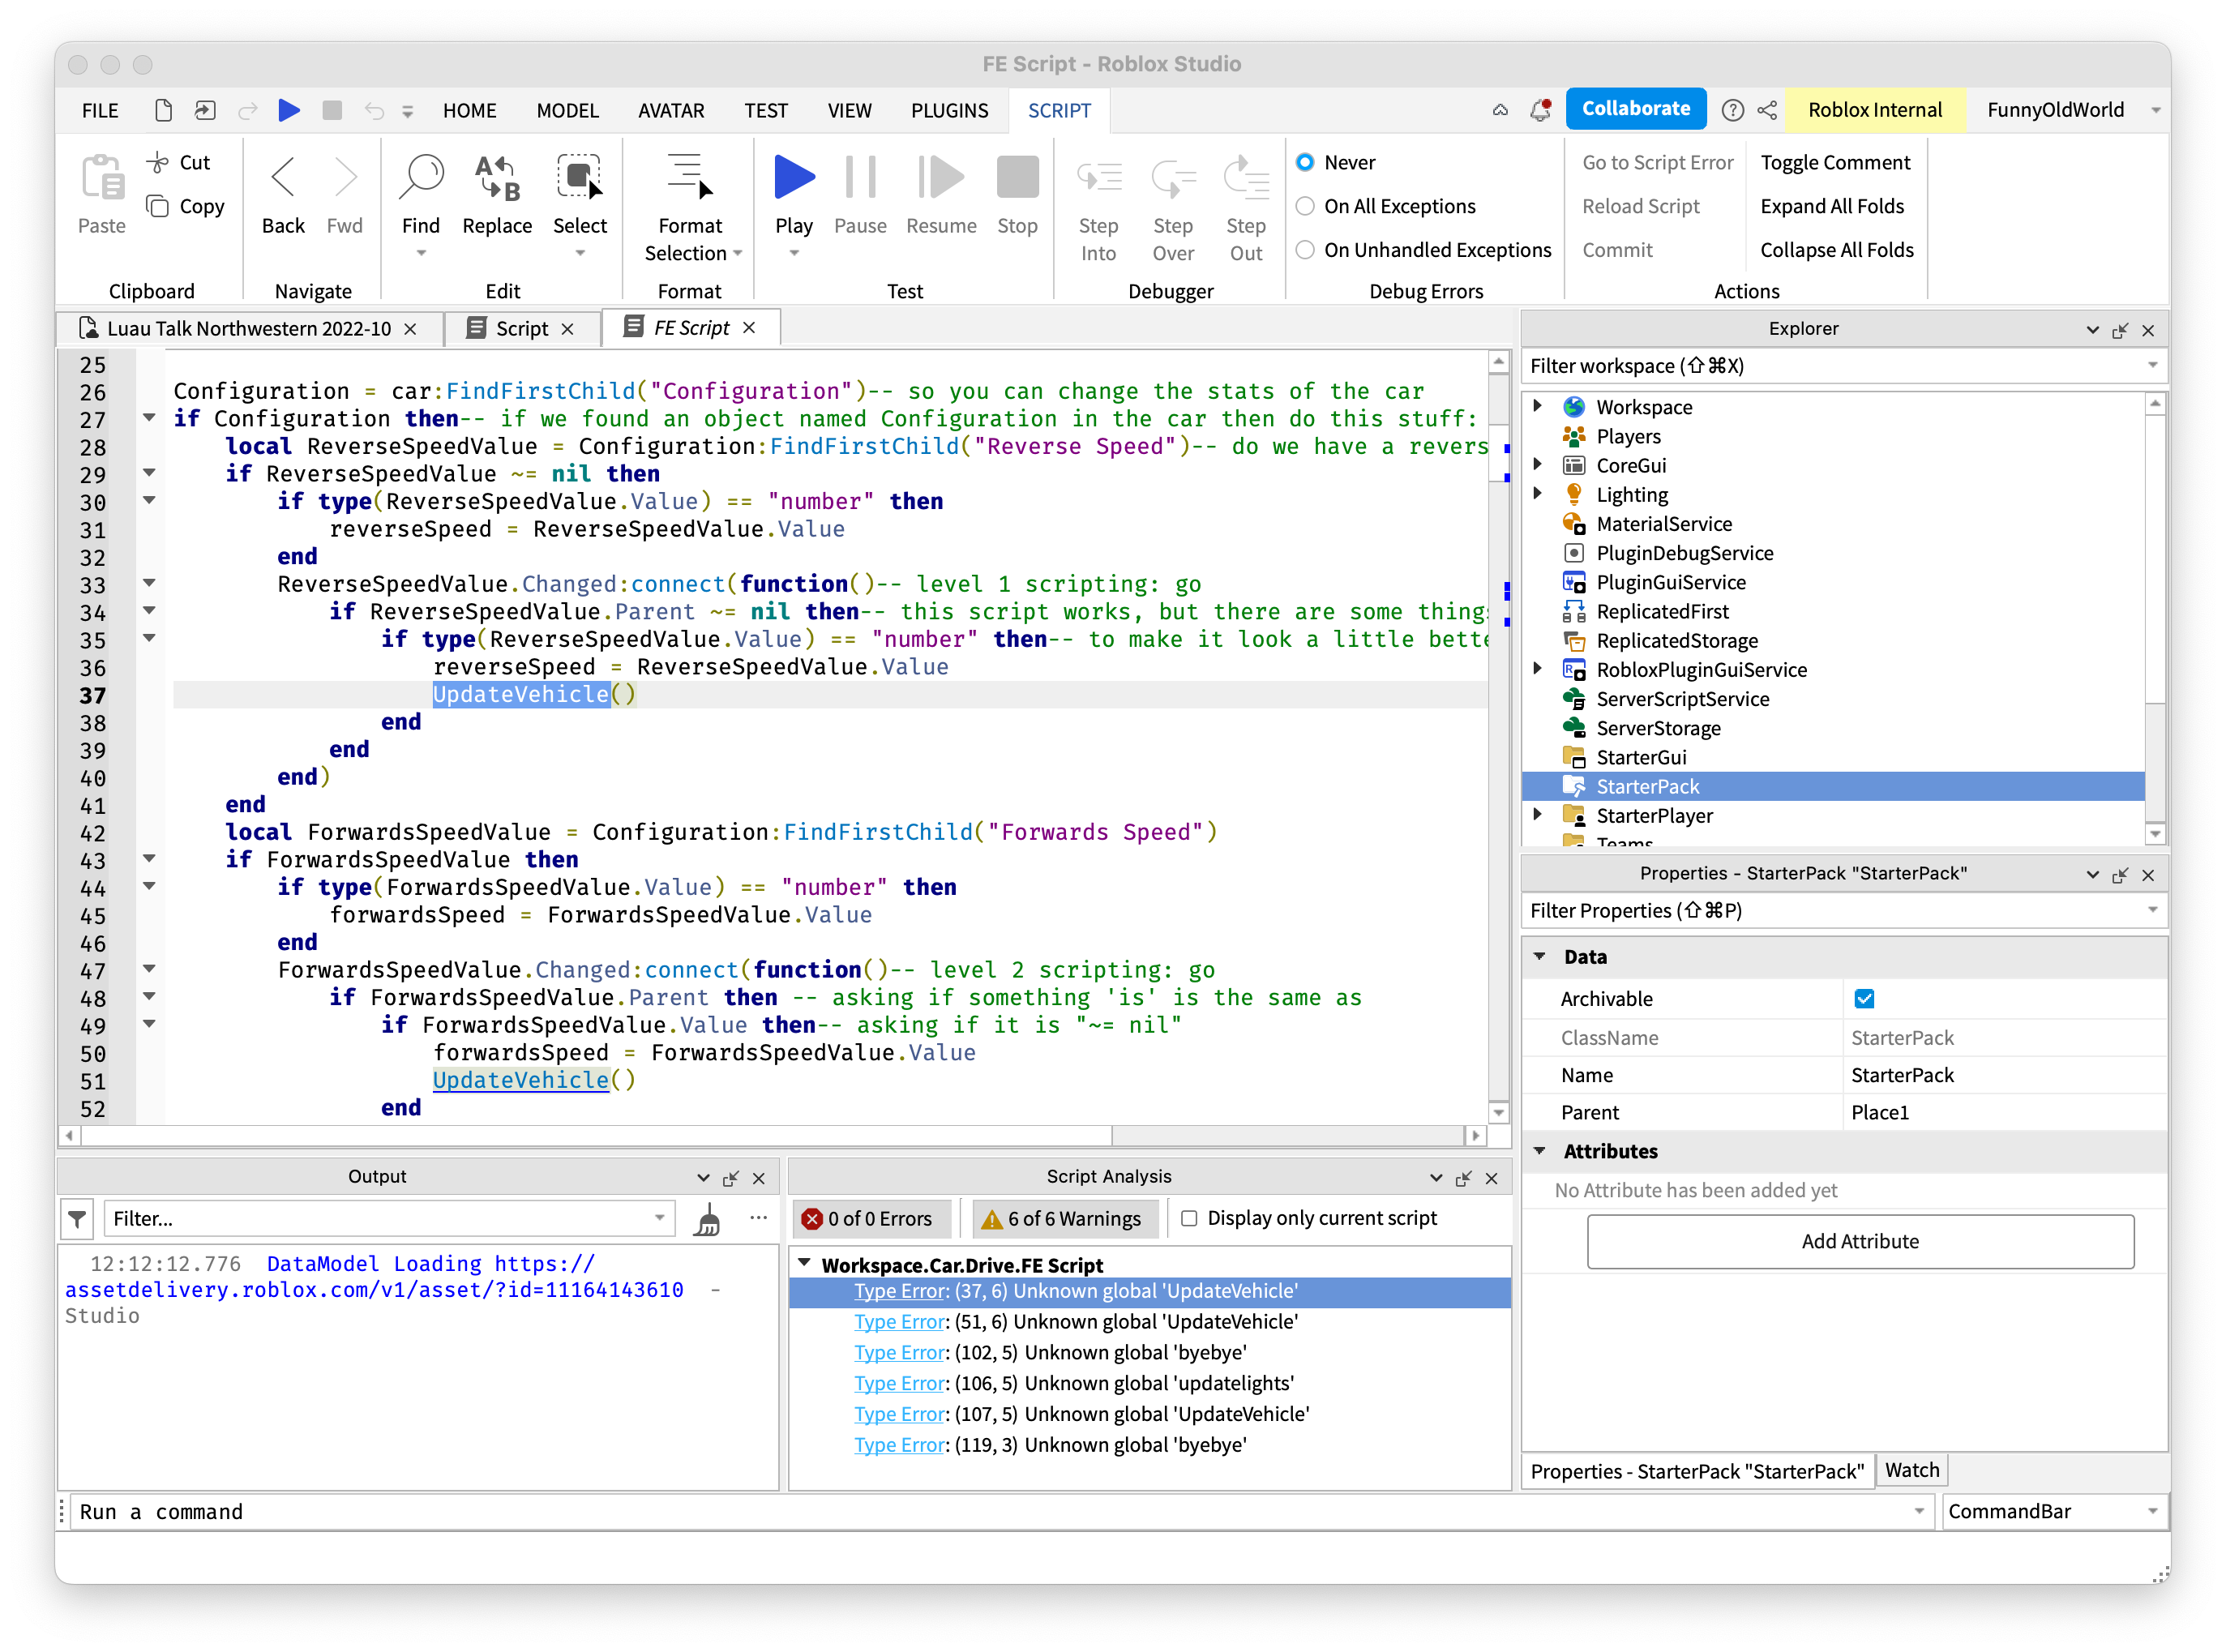
\includegraphics[width=.45\textwidth]{img/roblox-studio-ide.png}

  \caption{{Roblox Studio 3D creation} tools (left) and IDE (right)}
  \label{fig:roblox-studio}
\end{figure}

Creators of {Roblox experiences} use {Roblox Studio},
which combines {3D creation} tools as well as an Integrated
Developer Environment (IDE), as seen in Fig.~\ref{fig:roblox-studio}.
The IDE includes an optional ``Script Analysis'' widget, which
reports syntax errors, type errors, and problems identified by
lint tools. The script editor also (optionally) highlights
the location in code where reported errors occur.
To opt in to type error reporting, creators set a \emph{mode}
for each script, which is one of:
\begin{itemize}
  \item \mnocheck{}: only syntax errors are reported,
  \item \mnonstrict{}: all syntax errors, and a subset of ``high confidence'' type errors, are reported, or
  \item \mstrict{}: all syntax errors and type errors, are reported.
\end{itemize}
As an example of nonstrict mode, the following program only reports one error:
\begin{verbatim}
  --!nonstrict
  local x = { p = 5, q = nil }
  if condition then x.q = 7 end
  local y = x.p + x.q --> no type error
  local z = x.r       --> "Key 'r' not found in table 'x'"
\end{verbatim}
but in strict mode it reports two:
\begin{verbatim}
  --!strict
  local x = { p = 5, q = nil }
  if condition then x.q = 7 end
  local y = x.p + x.q --> "Type 'nil' could not be converted into 'number'"
  local z = x.r       --> "Key 'r' not found in table 'x'"
\end{verbatim}
In cases like this, where it is undecidable whether there will be a run-time error,
strict mode errs on the side of reporting an error, and nonstrict mode errs on
the side of suppressing the error.

Both modes report the \verb|Key 'r' not found in table 'x'| error --
misspellings of property names are common enough to report in both
strict and nonstrict mode. See~\cite{bfj-hatra-2021}
for a more detailed discussion of the rationale for strict and nonstrict mode.

Both modes are opt-in. Creators have the option to make \mnonstrict{} mode
the default rather than \mnocheck{} mode.

Even in \mnocheck{} mode, {Roblox Studio} performs type inference, since
the results are needed by type-directed tooling such as autocomplete and
API documentation. This behind-the-scenes typechecking is always performed
in strict mode, since it is important that the inferred types be as precise
as possible. The type errors produced by this pass are always discarded,
so the verbosity of strict mode is not an issue.

Since this pass is always performed in strict mode, we refer to it as
\emph{forced strict} mode. Its main use is in autocomplete, so forced
strict mode is triggered on every keystroke

Scripts come in two favors: \emph{module scripts} and \emph{non-module
scripts}.  Module scripts provide reusable libraries, which may be
\emph{required} by other scripts. Since module scripts can require
other module script, modules form a graph (though it is
an error in strict mode if the graph is cyclic, and edges are removed to
make the graph acyclic).

When typechecking is performed for script analysis, any script that
has been modified is marked as dirty, then any script that is dirty,
or which transitively requires a dirty module, is typechecked. More
commonly, when typechecking is performed for autocomplete, only
the current script is typechecked, since it is the only dirty
script, and nothing it requires can transitively require it, since
the module graph is acyclic.

The state of the world in a {Roblox} experience is captured by
the \emph{data model}, which is a tree of \emph{instances}, such as
parts, models, meshes, effects, lighting, audio assets, and physics
constraints such as forces, springs and joints.
The data model can be seen in the Explorer view of Fig.~\ref{fig:roblox-studio}.
While an experience is under development, it is typical for the data
model to be edited (for example instances to be added, deleted, moved
or renamed). Since the initial shape of the data model tree is reflected in
the type system, it is possible for these edits to introduce type errors.

\begin{table}
  \caption{Selected Error Labels}
  %% from type analysis, but they're not all really type errors
  %% TODO review selection after analyzing the full data
  \label{t:type-error-labels}

  %% FILL examples for each error?
  \begin{tabular}{ll}
    Label & Interpretation \\\midrule
    \code{CodeTooComplex} & Type analysis failed, cannot understand the code\!\!\! \\
    \code{UnificationTooComplex} & Type analysis failed, unification solver hit a limit\!\!\! \\
    \code{SyntaxError} & Basic parse error, e.g., \code{for if end} \\

    \code{CountMismatch} & Arity mismatch for a function \\
    \code{IncorrectGenericParameterCount} & Arity mismatch for a generic type \\
    \code{UnknownProperty} & Referenced an invalid field or method  \\
    \code{OnlyTablesCanHaveMethods} & Tried to attach a method to a non-table \\
    \code{CannotCallNonFunction} & Called a value that is not a function \\
    \code{TypesAreUnrelated} & Failed to cast, unify, or check subtyping \\
    \code{TypeMismatch} & Generic label for other type errors \\
    \code{GenericError}
    & Generic label for other non-type errors, such as\\
    & \hbox{}~~looping over an unordered table
    %% attempting to extend a type that does not describe a class
    %% attempting to iterate over a table without a clear order


%    \code{ExtraInformation} & Follow-on error that provides additional information for an error at the same source location. \\
%    UnknownSymbol &  \\
%    NotATable &  \\
%    CannotExtendTable &  \\
%    DuplicateTypeDefinition &  \\
%    FunctionDoesNotTakeSelf &  \\
%    FunctionRequiresSelf &  \\
%    OccursCheckFailed &  \\
%    UnknownRequire &  \\
%    UnknownPropButFoundLikeProp &  \\
%    InternalError &  \\
%    DeprecatedApiUsed &  \\
%    ModuleHasCyclicDependency &  \\
%    IllegalRequire &  \\
%    FunctionExitsWithoutReturning &  \\
%    DuplicateGenericParameter &  \\
%    CannotInferBinaryOperation &  \\
%    MissingProperties &  \\
%    SwappedGenericTypeParameter &  \\
%    OptionalValueAccess &  \\
%    MissingUnionProperty &  \\
%    NormalizationTooComplex &  \\
%    TypePackMismatch &  \\
%    DynamicPropertyLookupOnClassesUnsafe &  \\)
  \end{tabular}
\end{table}

\section{Telemetry Design}

\subsection{Limits of telemetry}

Telemetry allows an application to ``phone home'' with data
summarizing usage patterns, such performance data, crash reporting,
and feature uptake. A typical usage is in deciding whether an API can
be deprecated: without telemetry it may be difficult to know how
popular a feature is with users, but with telemetry it is
straightforward.

IDEs use telemetry in a similar fashion to most user-facing
applications, for example VSCode~\cite{vsc-telemetry} and
IntelliJ~\cite{intellij-telemetry} report telemetry.
See~\cref{s:related} for futher comparisons among telemetry designs.

Telemetry for programming languages can be controversial, for example
the lively discussion around telemetry in the Go
toolchain~\cite{golang-telemetry}. 
The Luau open source toolchain does \emph{not} report telemetry,
as it is designed to be used in build environments such as Continuous Integration
servers, where hermetic deterministic builds are expected.

Much of the concern about telemetry is because of its potential impact on
privacy, by revealing Personally Identifiable Information (PII).
For this reason, it is important that any experiments using telemetry
not reveal PII:
no source code;
no source code locations;
no error messages (which may contain source code);
no record of the creator's identity, locale, or IP address;
and no information about what creation the data came from.
A good introduction to the privacy implications and tradeoffs
involved with telemetry is~\cite{transparent-telemetry}.

For performance reasons, there are limits to telemetry data:
telemetry records have size limits, and the performance impact of
recording telemetry should be minimal.

In summary, the limitations of telemetry are:
\begin{itemize}
  \item Data which reveals no PII.
  \item Fixed-size telemetry records.
  \item Minimal overhead to record telemtry.
\end{itemize}
In addition, due to the architecture of Roblox Studio
there is some information that is not available to the
typechecker:
\begin{itemize}
  \item The typechecker does not have access to some lifecycle events,
    such as save, quit and publish.
  \item The typechecker does not have access to GUI state, for example
    whether the Script Analysis widget is visible.
\end{itemize}

\subsection{Telemetry records}
\label{s:telemetry-records}

The telemetry for a Roblox Studio session is gathered as a series of
telemtry records, all with the same psedonynimized session
identifier. This allows us to correlate telemetry across a single
session, but not between sessions.

In order to avoid swamping our telemetry servers, we randomly throttle
the generation of telemetry records:
\begin{itemize}
  \item
    1\% of Roblox Studio sessions were enrolled in generating telemetry, and
  \item
    0.5\% of runs of the typechecker (approximately 1 in 200 keystrokes)
      in an enrolled session generated a telemetry record.
\end{itemize}
In order to find how file-switching correlated with type errors, we additionally have:
\begin{itemize}
  \item
    every run of the typechecker in an enrolled session which switched file generated a telemetry record.
\end{itemize}
Each telemetry record contains:
\begin{description}
  \item[D1] metadata: a psedonymized session identifier, timestamp and session duration,
  \item[D2] mode of the current file: (\mnocheck{}, \mnonstrict{}, or \mstrict{}),
  \item[D3] reason for sending: (random selection, or file switch),
  \item[D4] size of codebase: number of files, and number of lines of code type checked,
  \item[D5] size of edit range
  \item[D6] overall type errors: for previous and current states, we have the total number, the nunber in the current file, and number in the edit range,
  \item[D7] specific errors in the edit range: for the previous and current states, for each type error code, the number type errors in the edit range,
  \item[D8] forced strict errors: specific errors for the
    edit range computed as if the user had strict mode enabled.
  \item[D9] TooComplexErrors: project-wide count for this one specific error type
\end{description}
To track the edit range, we record a start and end position, which we
update appropriately on every edit. This can result in very large edit
ranges, for example, if the user edits at the beginning and end of the
file.
The main benefit of this strategy is that it ensures constant-size telemetry records.


%%%%%%%%%%%%%%%%%%%%%%%%%%%%%%%%%%%%%%%%%%%%%%%%%%%%%%%%%%%%%%%%%%%%%%%%%%%%%%%%%%%%%%%%%%%%%%%%%%%
%%%  STOP!  ROUGH TEXT BELOW     %%%%%%%%%%%%%%%%%%%%%%%%%%%%%%%%%%%%%%%%%%%%%%%%%%%%%%%%%%%%%%%%%%
%%%%%%%%%%%%%%%%%%%%%%%%%%%%%%%%%%%%%%%%%%%%%%%%%%%%%%%%%%%%%%%%%%%%%%%%%%%%%%%%%%%%%%%%%%%%%%%%%%%

\section{The Data}
\label{s:data}

Roblox Studio collected type error telemetry in Spring 2023,
between February and April.
Every Studio session had a small random chance of generating
telemetry~(\cref{s:telemetry-records}).
The chosen sessions generated a record whenever the user switched modules and
randomly on each keystroke.

\Cref{f:records-per-hour} provides a time-ordered distribution of the data.
Each vertical bar counts the number of records generated per hour according to
a client-side timestamp.
The bars are labeled with a California time zone because that is the locale of
the Roblox servers, which parsed the timestamps.
Most buckets contain roughly one thousand records, but some have very few
and a handful of others exceed three thousand.
%% \FILL{} investigate one tower, what's happening?? all one session?
There is a sharp drop in early April because we disabled telemetry at that point
but some clients continued to generate data
(\FILL{} Q. Alan, is that an ok sentence? I'm not sure why there's a long tail,
guess it could be people not updating studio or people with strange time settings
on their machine.)
We do not know which timezone the records originated in, but since the counts
tend to peak midday California time it seems that the majority
of Roblox developers are following a Western Hemisphere schedule.
%% \FILL{} probably North America, but do we really want to guess?
The counts for weekends (shaded regions) are often the tallest; these days presumably
have a larger number of sessions for telemetry to observe.

\begin{figure}[t]
  %% TODO bigger text
  %% TODO weird artifact (|) in x-min label
  %% code/row-distribution.rkt
  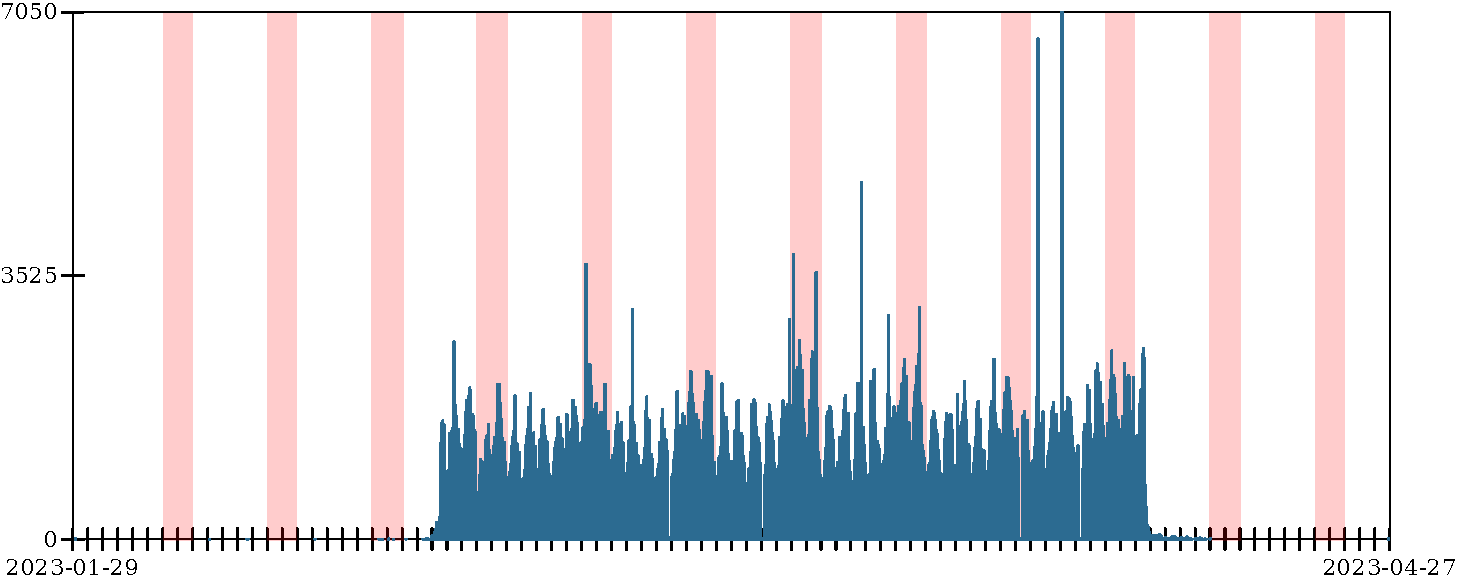
\includegraphics[width=\columnwidth]{img/row-distribution.pdf}
  \caption{Telemetry records per hour. Each tick on the $x$-axis marks the start of a new day in California. Shaded ranges correspond to weekends.}
  \label{f:records-per-hour}
\end{figure}


\subsection{Data Cleaning}
\label{s:data-cleaning}

A close inspection of the data revealed a few anomalies.
For the most part, we omit the strange data from futher analysis.

First, some records have odd timestamps according to the server's records.
Every telemetry record comes with two timestamps: a client-side timestamp
from when Roblox Studio created it and a server-side timestamp from when
the server posted it to its database.
The server timestamps are little use for our analysis because they bunch
together; it is common for several records to have identical server
timestamps.
However, server timestamps are useful for auditing because they should
be relatively close in value to the client timestamps.
For some records (<100? \FILL{}), though, the client is off by a large
margin: up to one week behind and up to one day ahead of the server.
We attribute the large delays to issues when sending telemetry (lost internet
connection, etc.) and smaller offsets to incorrect time settings on the client
machine.
In any event, we do not filter these records from further analysis.

Second, some records have identical (client) timestamps.
This can happen legitimately if type analysis runs several times
in the same millisecond, but it is unlikely that a human would
enter keystrokes or switch modules quickly enough.
We keep the first record with a distinct timestamp and discard the others.
%% TODO wait, better deduplicate by session and not globally!!!

%% out/negative-edit-range.txt
%% actual value is NOT negative, but large positive over 4 billion
%% example: 4294967293
Third, the edit ranges are negative in a few hundred records~(1,533).
This is likely due to the user deleting a large block of code.
Since the issue affects so few records, we omit the negative ranges
from analysis (but, we do use other parts of the records; for example
the timestamps influence~\cref{f:records-per-hour}).
(\FILL{} Alan, double-check reasoning)


\subsection{Codebase Size}
\label{s:codebase-size}

\begin{figure}[t]
  % ;; (list* (max* vv) (median < vv) mm (stddev/mean mm vv) (percentile* vv)))
  % ;; percentile* = 0.95 -- 0.99
  %#hash((editrange . (1156036 926 3007043/817 30975.40553032358 (0.95 8220) (0.96 9858) (0.97 13656) (0.98 18956) (0.99 34725)))
  %      (event-count . (6079 138 38689/135 582.5752201972966 (0.95 960) (0.96 1174) (0.97 1304) (0.98 1836) (0.99 3302)))
  %      (files . (54884 7678 55257996/4639 11853.650098459446 (0.95 40029) (0.96 42771) (0.97 45417) (0.98 48688) (0.99 51761)))
  %      (lines . (1089963 3115 38928947/5992 22364.75846303099 (0.95 18561) (0.96 25892) (0.97 27014) (0.98 29725) (0.99 50547)))
  %      (timespan . (1387897376 845648 591343604248/185705 15724745.722577972 (0.95 10696064) (0.96 12715468) (0.97 15596940) (0.98 21153924) (0.99 35450460))))
  %% NOTE: 3 records have +1M lines, all from one nocheck session, all with 3 files
  %% - session "30,762,216,447,324"
  %% NOTE: 133 records have +52K files, all from one nocheck session
  %% - session "330,172,870,224,081" 
  %% (2nd biggest has 41K files "31,650,473,913,529")

  \begin{tabular}{l@{}r@{~}l@{}r@{~}l@{}r@{~}l}
                 & Files  &              &     Lines &             &    Edit Range & \\
    Mean [std]   & 11,911 & \stddev{31}  &     6,497 & \stddev{22} &         3,680 & \stddev{12} \\
    Median       &  7,678 &              &     3,115 &             &           926 & \\
    \pct{99}     & 51,761 &              &    50,547 &             &        34,725 & \\
    & 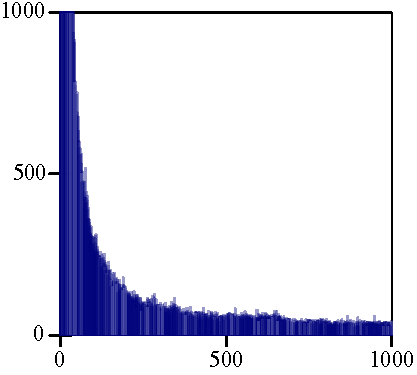
\includegraphics[width=0.2\columnwidth]{img/files-distribution.pdf}
    & & 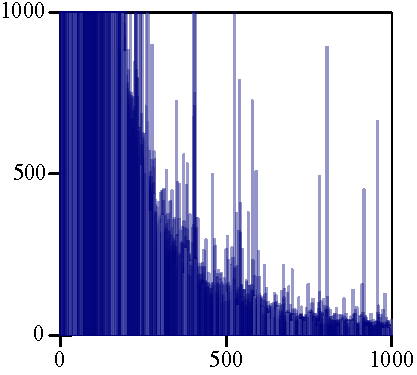
\includegraphics[width=0.2\columnwidth]{img/lines-distribution.pdf}
    & & 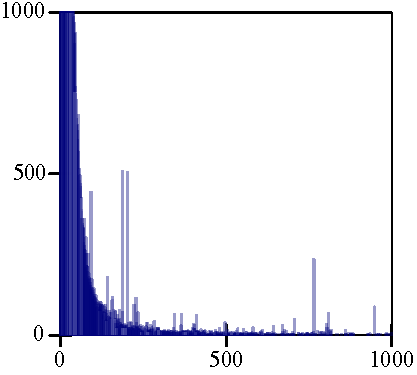
\includegraphics[width=0.2\columnwidth]{img/editrange-distribution.pdf}

  \end{tabular}

  \caption{Size of analyzed code: number of files, number of lines , and lines in edit range}
  \label{f:codebase-size}
\end{figure}

TODO findings lessons etc.


FILL power-law files lines editrange.
Incredible max numbers.


\subsection{??? records}

\begin{figure}[t]
  \begin{subfigure}[t]{\columnwidth}
    \begin{tabular}[t]{ll}
      \begin{tabular}[t]{r@{~~}l@{~}r}
         1,341,348 & \mnocheck{}          & [\pct{89.14}] \\
           156,883 & \mnonstrict{}        & [\pct{10.43}] \\
             6,505 & \mstrict{}           & [\pct{ 0.43}]
      \end{tabular}
      \begin{tabular}[t]{r@{~~}l@{~~}r}
           508,572 & due to module switch & [\pct{33.80}] \\
           996,164 & due to keystrokes    & [\pct{66.20}]
      \end{tabular}
    \end{tabular}
    \caption{Total telemetry records (1,504,736), analysis modes, and reason-for-sending}
    \label{f:total-records}
  \end{subfigure}

  \begin{subfigure}[t]{\columnwidth}
    \begin{tabular}[t]{ll} \\
      \begin{tabular}[t]{l@{~~}r@{~}l}
        595,137 & Type errors \\
        289,698 & in current module & [\pct{48.68}] \\
         30,924 & in edit range & [\pct{5.20}]
      \end{tabular}
      \begin{tabular}[t]{l@{~~}r@{~}l}
        72,235,735 & {Forced-strict errors} \\
        37,027,281 & in current module & [\pct{51.26}] \\
         1,111,178 & in edit range & [\pct{1.54}]
      \end{tabular}
    \end{tabular}
    \caption{Type errors and forced-strict errors across all telemetry records}
    \label{f:total-tefs}
  \end{subfigure}

  \begin{subfigure}[t]{\columnwidth}
    \begin{tabular}[t]{ll} \\
      \begin{tabular}[t]{l@{~~}r@{~}l}
        313,509 & \mnocheck{}   & [\pct{90.19}] \\
         32,902 & \mnonstrict{} & [\pct{ 9.47}] \\
            545 & \mstrict{}    & [\pct{ 0.16}] \\
            642 & mixed-mode    & [\pct{ 0.18}]
      \end{tabular}
      \begin{tabular}[t]{l@{~~}ll}
        \zerowidth{Among the mixed-mode sessions:} \\
        & 341 & contain a mode upgrade \\
        & 320 & contain a mode downgrade \\
        & 512 & contain modules with different modes
      \end{tabular}
    \end{tabular}
    \caption{Total sessions (347,598), whether and how they switch analysis mode}
    \label{f:total-sessions}
  \end{subfigure}

  \begin{subfigure}[t]{\columnwidth}
    %% NOTE max time = 1 million seconds = 15 days ...  +100 are over 2 days

    \begin{tabular}{l@{}r@{~}l@{}r@{~}l} \\
                   & Time Span (sec)  &       & Record Count  \\
      Mean [std]   &     3,184 & \stddev{16}  &     286 & [583] \\
      Median       &       845 &              &     138        \\
      \pct{99}     &    35,450 &              &   3,302        \\
      & 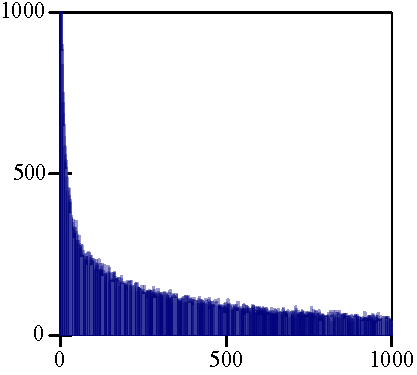
\includegraphics[width=0.2\columnwidth]{img/timespan-distribution.pdf}
      & & 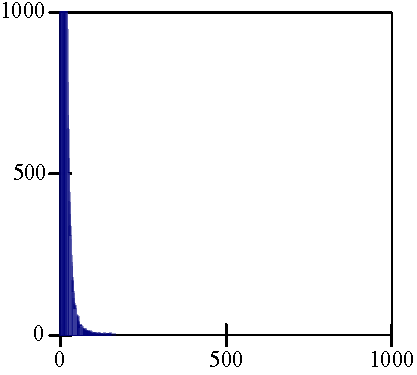
\includegraphics[width=0.2\columnwidth]{img/event-count-distribution.pdf}

    \end{tabular}

    \caption{Session length in seconds and in number of records}
    \label{f:sessions-size}
  \end{subfigure}

  \caption{Dataset overview}
  \label{f:dataset-overview}
\end{figure}

\Cref{f:dataset-overview}

FILL nocheck nonstrict strict, order-of-magnitude

FILL type error counts
Mostly syntax errors though!
Estimate \pct{40} are substantial type errors rather than syntax
errors based on the edit range type errors~(\cref{s:type-error-count})
but unfortunately we cannot get an exact number for the overall
or per-module type error counts.

FILL single-mode sessions, mostly

FILL details on upgrades, downgrades, then ignore these for rest of paper.
multi-mode project = found a module switch that coincides with a mode switch, which suggests that two modules have different modes;
upgrade = found a up-mode switch that does not match a module switch (quite possible to miss these);
downgrade = found a down-mode switch that does not match a module switch

wow 619 up-pairs, 583 down-pairs
=== UP
min -3 max 57 median 0 mean 2.62 stddev 6.8390518952707335
=== DOWN
min -48 max 30 median 0 mean -0.31 stddev 4.498748355271854


FILL most sessions fairly long in time (order of minutes),
short in event count (dozens).


\section{Type Errors in Edit Range}
\label{s:type-error-count}

\begin{table}[t]
  \caption{Type error survival}
  \label{t:type-error-survival}

    \begin{tabular}{lr@{}r@{}rr@{}r@{}rr@{}r@{}r}
      & \zerowidth{\mnocheck{}} & & & \zerowidth{\mnonstrict{}} & & & \zerowidth{\mstrict{}} & & \\
      & \rbox{Add} & \ybox{Keep} & \gbox{Drop} & \rbox{Add} & \ybox{Keep} & \gbox{Drop} & \rbox{Add} & \ybox{Keep} & \gbox{Drop} \\\midrule
      TypeMismatch & {0} & {0} & {0} & {159} & {62} & {129} & {21} & {10} & {28} \\
      UnknownSymbol & {0} & {0} & {0} & {2348} & {496} & {2973} & {49} & {19} & {55} \\
      UnknownProperty & {0} & {0} & {0} & {347} & {180} & {385} & {19} & {19} & {35} \\
      NotATable & {0} & {0} & {0} & {7} & {2} & {8} & {2} & {0} & {1} \\
      CannotExtendTable & {0} & {0} & {0} & {7} & {9} & {10} & {0} & {0} & {1} \\
      OnlyTablesCanHaveMethods & {0} & {0} & {0} & {1} & {0} & {2} & {0} & {0} & {0} \\
      DuplicateTypeDefinition & {0} & {0} & {0} & {1} & {0} & {0} & {0} & {0} & {0} \\
      CountMismatch & {0} & {0} & {0} & {223} & {48} & {269} & {12} & {2} & {17} \\
      FunctionDoesNotTakeSelf & {0} & {0} & {0} & {4} & {6} & {5} & {0} & {0} & {0} \\
      OccursCheckFailed & {0} & {0} & {0} & {0} & {0} & {0} & {0} & {0} & {1} \\
      UnknownRequire & {0} & {0} & {0} & {91} & {39} & {85} & {12} & {3} & {4} \\
      IncorrectGenericParameterCount & {0} & {0} & {0} & {0} & {0} & {0} & {1} & {0} & {1} \\
      SyntaxError & {8349} & {314} & {19220} & {983} & {46} & {2658} & {16} & {0} & {71} \\
      UnknownPropButFoundLikeProp & {0} & {0} & {0} & {26} & {18} & {21} & {1} & {0} & {1} \\
      GenericError & {0} & {0} & {0} & {206} & {52} & {203} & {8} & {1} & {9} \\
      CannotCallNonFunction & {0} & {0} & {0} & {17} & {4} & {20} & {1} & {0} & {1} \\
      ExtraInformation & {0} & {0} & {0} & {48} & {7} & {39} & {2} & {0} & {1} \\
      ModuleHasCyclicDependency & {0} & {0} & {0} & {20} & {9} & {15} & {0} & {0} & {1} \\
      IllegalRequire & {0} & {0} & {0} & {16} & {3} & {33} & {0} & {0} & {2} \\
      FunctionExitsWithoutReturning & {0} & {0} & {0} & {9} & {3} & {6} & {11} & {5} & {8} \\
      CannotInferBinaryOperation & {0} & {0} & {0} & {1} & {2} & {1} & {7} & {6} & {9} \\
      MissingProperties & {0} & {0} & {0} & {11} & {3} & {11} & {6} & {4} & {6} \\
      OptionalValueAccess & {0} & {0} & {0} & {40} & {52} & {27} & {6} & {2} & {7} \\
      MissingUnionProperty & {0} & {0} & {0} & {1} & {0} & {2} & {0} & {0} & {0} \\
      TypesAreUnrelated & {0} & {0} & {0} & {1} & {0} & {0} & {0} & {0} & {1} \\
    \end{tabular}

\end{table}

FILL popularity over all old and new in edit range.
Syntax error by far the most common.
UnknownSymbol is likely a syntax error --- so \pct{90} syntax error!

FILL N errors never showed up.
Nothing for \code{CodeTooComplex} or \code{UnificationTooComplex} is great news.
But what about the others? FILL

TODO get counts for each mode. Are there fewer stx errors in strict mode??!

NOTE can't ask about type errors at end because we don't know
the end.
The final record can be sent minutes before the end of session.


\begin{table}[t]\centering
  %% NOTE: popularity looks similar when [over all records] vs. [restricted to module switch records]

  \begin{tabular}{ll}
    \mnonstrict{} & \mstrict{} \\
    \begin{tabular}[t]{l@{~}r}
      \code{UnknownSymbol} & \pct{62.13} \\
      \code{SyntaxError} & \pct{15.42} \\
      \code{UnknownProperty} & \pct{8.28} \\
      \code{UnknownRequire} & \pct{3.13} \\
      \code{TypeMismatch} & \pct{2.44} \\
      \code{CountMismatch} & \pct{2.26} \\
      \code{OptionalValueAccess} & \pct{2.07} \\
      \code{GenericError} & \pct{2.06} \\
      \code{UnknownPropButFoundLikeProp} & \pct{0.44} \\
      \code{CannotExtendTable} & \pct{0.42} \\
      \code{ExtraInformation} & \pct{0.32} \\
      \code{ModuleHasCyclicDependency} & \pct{0.23} \\
      \code{IllegalRequire} & \pct{0.20} \\
      \code{NotATable} & \pct{0.15} \\
      \code{CannotCallNonFunction} & \pct{0.15} \\
      \code{MissingProperties} & \pct{0.09} \\
      \code{FunctionExitsWithoutReturning} & \pct{0.07} \\
      \code{FunctionDoesNotTakeSelf} & \pct{0.07} \\
      \code{MissingUnionProperty} & \pct{0.02} \\
      \code{CannotInferBinaryOperation} & \pct{0.02} \\
      \code{OnlyTablesCanHaveMethods} & \pct{0.01} \\
      \code{DuplicateTypeDefinition} & {<\pct{0.01}} \\
      \code{TypesAreUnrelated} & {<\pct{0.01}} \\
    \end{tabular}
        &
    \begin{tabular}[t]{l@{~}r}
      \code{UnknownSymbol} & \pct{23.97} \\
      \code{TypeMismatch} & \pct{20.46} \\
      \code{UnknownProperty} & \pct{18.88} \\
      \code{SyntaxError} & \pct{9.31} \\
      \code{CannotInferBinaryOperation} & \pct{6.94} \\
      \code{MissingProperties} & \pct{4.04} \\
      \code{CountMismatch} & \pct{2.99} \\
      \code{OptionalValueAccess} & \pct{2.99} \\
      \code{FunctionExitsWithoutReturning} & \pct{2.99} \\
      \code{UnknownRequire} & \pct{2.37} \\
      \code{GenericError} & \pct{2.28} \\
      \code{NotATable} & \pct{1.32} \\
      \code{ExtraInformation} & \pct{0.35} \\
      \code{UnknownPropButFoundLikeProp} & \pct{0.26} \\
      \code{IncorrectGenericParameterCount} & \pct{0.18} \\
      \code{CannotCallNonFunction} & \pct{0.18} \\
      \code{IllegalRequire} & \pct{0.18} \\
      \code{ModuleHasCyclicDependency} & \pct{0.09} \\
      \code{CannotExtendTable} & \pct{0.09} \\
      \code{OccursCheckFailed} & \pct{0.09} \\
      \code{TypesAreUnrelated} & \pct{0.09} \\
    \end{tabular}
  \end{tabular}

  \caption{Type error popularity for \mnonstrict{} and \mstrict{} modes.
  In \mnocheck{}, \code{SyntaxError} accounts for \pct{100} of the error.}
  \label{t:type-error-count}
\end{table}


\section{Analysis}

\subsection{Analysis 2}

TODO work this into the above or below.

What can we learn from the telemetry? We have 1.5 million records from Feb 22
to April 14 (roughly 27K records per day).
They mention +70 million type errors.
(Some records point to a large number of errors. FILL median, max. Could be cascading,
which makes the 70million number uninterpretable.)
What takeaways are there??!

First,
users rarely switch type analysis mode. There are 3 modes available and users
are free to switch between them, or to mix modes in a codebase, but we rarely
detect these events:

\pct{99} of sessions use a single mode

\pct{0.2} of sessions use different modes in different modules. (More
precisely, the user switched to a module --- triggering a telemetry record ---
that used a different mode than the previous one.)

\pct{0.2} of records show a mode switch (equally split between upgrades and
downgrades, 341 and 320)


Second,
the stronger analysis modes are roughly 10x less popular than weaker ones
(across the \pct{99} of sessions that stick with one mode):

\pct{90} of sessions use nocheck mode
\pct{9.8} use nonstrict mode
\pct{0.2} use strict mode

Third,
In the edit range, we know exactly which errors showed up. This leads to a few
takeaways, such as:

Only 3 sessions (out of +300K) hit the typechecker's internal limits on problem
size --- CodeTooComplex errors. Good!

About \pct{90} of type errors are probably due to typos (SyntaxError, UnknownSymbol,
UnknownProperty). These are not propoer type errors.

10 errors never showed up. These include DynamicPropertyLookupOnClassesUnsafe and
SwappedGenericTypeParameter


Fourth,
Codebase size and session length tend to follow a power law. 
One aspect of size for nonstrict sessions: the number of
lines in the edit range. Over 80 sessions have 20-line ranges, about 40 have a
30-line range, etc.

Fifth,
Increases and decreases to the number of type errors are evenly balanced across
the data.
In strict mode, \pct{24} of records increase the number of type errors. \pct{26}
decrease. \pct{50} keep it constant.
In nonstrict mode, \pct{14} increase errors, \pct{15} decrease, and \pct{71}
keep it constant
This plot is for nonstrict. X-axis = time since start of session, cut off at 30
seconds. Y-axis = change in num errors since last record, cut off at +/- 100.

\begin{figure}[t]\centering
% TODO diff vs 1st, not previous

  \mnocheck{}
  \includegraphics[width=\columnwidth]{img/error-count-nocheck-row--te-density-diff.pdf}
  \medskip
  \mnonstrict{}
  \includegraphics[width=\columnwidth]{img/error-count-nonstrict-row--te-density-diff.pdf}
  \medskip
  \mstrict{}
  \includegraphics[width=\columnwidth]{img/error-count-strict-row--te-density-diff.pdf}

  TODO bars instead, percent only, don't care about counts

  \begin{tabular}{lr@{}rr@{}rr@{}r}
    & \zerowidth{Add} & & \zerowidth{Keep} & & \zerowidth{Drop} \\\midrule
    \mnocheck{} & 48378 & [\pct{46.83}] & 9440 & [\pct{9.14}] & 45479 & [\pct{44.03}] \\
    \mnonstrict{} & 19491 & [\pct{39.63}] & 9567 & [\pct{19.45}] & 20121 & [\pct{40.91}] \\
    \mstrict{} & 733 & [\pct{39.18}] & 368 & [\pct{19.67}] & 770 & [\pct{41.15}] \\
  \end{tabular}
  \caption{FILL error density}
  \label{f:error-delta}
\end{figure}

Sixth, DM story.
FS has: 1 all dependencies in strict, 2 data-model awareness (DM turns into
type graph, ... initial DM, all properties go into a table type; DM -> folder
-> model -> part .. get dot-driven autocomplete) in strict, DM might have type
Any might have type Instance, the latter would mean more errors than FS

DM insensitivity in strict mode
(if DM has top type that would lead to errors.)
Context: each of the 3 modes runs 2 kinds of type analysis. One is the regular
type analysis. The other is Forced Strict (FS), which converts all dependencies
to strict mode. The reason for FS is that it sometimes gives better
autocomplete suggestions etc.
You'd expect that the number of type errors is always <= num FS errors. But we
found several cases where this is false!
The plot here "stacks" every strict session into bars. X-axis is a record index
within a session (bars are higher on the left because we have lots more short
sessions than long ones). Y-axis counts the number of records where num TE <= num FS
is true (blue) and false (yellow).

\begin{figure}[t]\centering
  %% TODO
  %% - thin bars
  %% - colors for good , bad (disagree) , neutral
  \begin{tabular}{lll}
    \mnocheck{} & \mnonstrict{} & \mstrict{} \\
    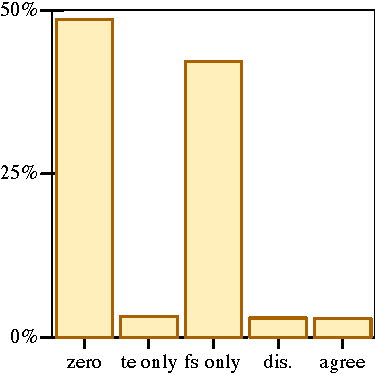
\includegraphics[width=0.3\columnwidth]{img/compass-nocheck.pdf}
    &
    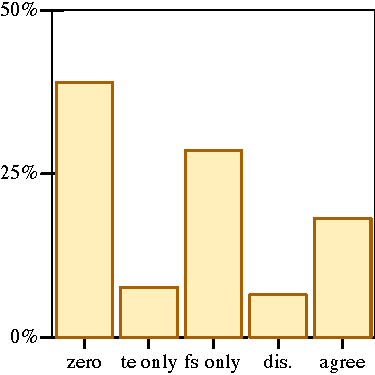
\includegraphics[width=0.3\columnwidth]{img/compass-nonstrict.pdf}
    &
    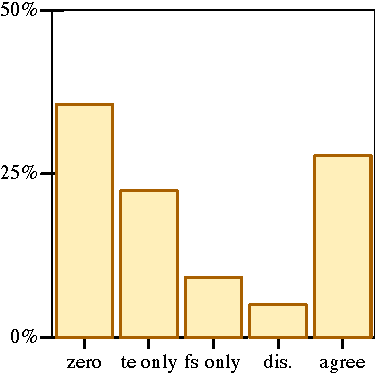
\includegraphics[width=0.3\columnwidth]{img/compass-strict.pdf}
  \end{tabular}
  \caption{FILL Are there fewer type errors than forcedstrict errors? Expect true always, but that is not the case.}
  \label{f:tefs}
\end{figure}

\Cref{f:tefs}~FILL story is edits to DM vs edits to code.
Data model awareness, call for future work.

\begin{figure}[t]\centering
  %% TODO can we 
  \mnonstrict{}\\
  \includegraphics[width=\columnwidth]{img/timeline-nonstrict.pdf}

  \medskip{}
  \mstrict{}\\
  \includegraphics[width=\columnwidth]{img/timeline-strict.pdf}

  \caption{Example sessions}
  \label{f:indy-session}
\end{figure}

TODO correlations, compare modes!!!


\section{Interpretation}

\subsection{Internal Error}
%% out/te-editrange-*

FILL hope to never see \code{InternalError}.
Have zero, yay!


\subsection{Dead Ends: Too Complex}
%% data = out/ctc-info.txt

To deal with pathologies such as the worst-case time for ML-style type
inference~\cite{m-popl-1990,ktu-caap-1990}, the typechecker
has internal limits that restrict the problems it will attempt to solve.
Hitting a limit triggers one of the following errors:
\code{CodeTooComplex},
\code{NormalizationTooComplex}, or
\code{UnificationTooComplex}.
A casual user should never see these errors.

Fortunately, the data rarely contains too-complex errors.
There are zero \code{UnificationTooComplex} errors and only a
handful of \code{CodeTooComplex} errors.
%% 26 total
It is entirely possible that the \code{CodeTooComplex} errors came from
a single user, as they appear in eleven records (out of 1.5 million)
spread across three sessions.
At any rate, the overall number is low enough to suggest that the internal
limits are not posing barriers to typechecker adoption.


\subsection{TBD}

Error 1000 = type mismatch (subtyping etc);
1001 = unknown symbol;
\ldots

% https://github.com/Roblox/luau/blob/master/Analysis/include/Luau/Error.h


\begin{verbatim}
 require(foobar)
  foobar is a module script in the data model
 require(foo.bar.b)
  - could be edit in progress
  - could be renamed module
  - 
\end{verbatim}


\subsection{Module Switches}

FILL why study, what implications?

FILL need \%s out of all module switches.

How many module switches exit a module with errors?
\mnocheck{} 24, \mnonstrict{} 9, \mstrict{} 3.
Rare?
More common for forcedstrict:
 \mnocheck{} 190, \mnonstrict{} 16, \mstrict{} 2.

How many module switches go to a module with errors?
\mnocheck{} 70, nonstrict 9, strict 4
For FS: \mnocheck{} 400, \mnonstrict{} 39, \mstrict{} 6.


\subsection{Types and Quality of Life}

FILL error density: number vs range size

TODO nocheck accumulated errors?


\subsection{Example Sessions}

FILL example sessions.


\subsection{Asset Creation vs Scripting}

Data model. Point to discussion above.

Big fluctuations in errors.
FS disagrees with TE.
Probably data model!


\section{Threats to Validity}
\label{s:threats}

Error counts per-project and per-module include syntax errors.
Problematic, because syntax errors are uninteresting (easy to fix),
but common, which makes it likely that our per-keystroke telemetry (1/200) will record them.
Edit range has specific counts.
Next time, we should do that for the other aggregates.

Telemetry cannot replace user studies, as there is no way to measure
creator sentiment, but provide complementary data at scale.


\section{Related Work}
\label{s:related}

Liblit dissertation~\cite{liblit-thesis}

RAMSS workshop series.

Differential privacy for coverage analysis of software traces,
adds noise to traces,
hard because infinitely many traces,
use CFG abstraction of possible behaviors for callgraph analysis,
count sketch data structure~\cite{hlzbr-ecoop-2021}.

Nasko~\cite{zhlbr-cc-2020,zhlbr-oopsla-2020,hlzbr-ecoop-2021}

%% - zfstt-ieeesensors-2022
%% - lit review, benefits of static types
%%   http://danluu.com/empirical-pl/
%% - thomas kennedy .... generic usage monitoring ascilite 2003
%% - ahmadzadeh elliman higgins iticse 2005
%% - buffardi etal 2014 adaptive and social mechanisms
%% - bddf-icse-2016
%% -  sh edwards and jason snyder icer 2009 comparing effective and ineffective grading platform
%% - murphy etal sigcse 2009 Retina: helping students
%% - ESP workshop on empirical studies of programming
%%   https://dl.acm.org/doi/proceedings/10.1145/266399
%%   nothing sounds big ... empirical yes, large no
%% - Choppella Haynes IU TR 426
%% - Tip Dinesh tosem 2001

\cite{bgimgm-cse-2016}
study Java compiler error messages after an intervention, counting num errors,
counting repeats, counting per user

\cite{anna-russo-kennedy-ms-2006}
BitFit, web-based java ide log num hint requests num, result of check answer
requests num compile, num run, no code?! good we have the same constraint

\cite{ab-sigcse-2015}
frequency, time-to-fix, spread of errors
 (we can't do time)
parsing compile error + source code
 sometimes with custom parsers

\cite{m-masters-2016}
study errors in blackbox dataset,
 overwhelmingly syntax

\cite{bkmu-sigcse-2014}
blackbox, 100k users
source code, diffs
error line, column, message;
keep all comments EXCEPT one above the class declaration


\cite{bask-icer-2018}
2TB data, Java programs
18 publications survey, technical challenges in analysis
 most pubs analyze errors;
nobody asked:
 which exns do students encounter (what?! mccall kolling 2014)
 execution / editing timelines
(blackbox analysis tutorial in sigcse 2020 on a mini dataset, to help researchers start writing an analysis)


\cite{t-hatra-2021}
plan for a large user-centered study 
... not very deep, look at edit sequences, replay for errors


\cite{cdhhjklwya-hatra-2020}
evaluating the PLIERS design process (Coblenz etal 202X)
teaching students to use PLIERS; everyone ran a user study!
6 languages
 3 ran usability studies
recommend talk-alouds


\cite{gstf-hatra-2021}
liquid types for java
30 devs user study
 zoom

\cite{lfgc-pldi-2007}
typechecker never errors,
 calls a helper that looks for nearby programs that do typecheck
tested on
 10 students, 2yrs professional experience
 5 hw assignments
 2122 files collected;
won \pct{19}, lost \pct{17};
ill-suited for things like (let x = e1 in ....),
 change e1,
 use typechecker feedback to guide edits;
small data!


\cite{w-popl-1986}
reporting source, not detection
tested on 9 type errors
 all \emph{deletions}, such as forgetting to inject in an enum

\cite{sscwj-oopsla-2017}
NATE numerical analysis of type errors
5000 labeled programs
 errors from class, first fix


\cite{sjw-jfp-2018}
type error witness generation
4500 ill-typed student programs
 \pct{85} of time, synthesis works
 \pct{70} of time, locate source


\cite{h-dissertiation-2005}
constraint-based type inference;
general te criteria:
- target audience (novice / expert)
- output format (text / viz)
- interactivity (yes / no)
- heuristics (yes / no)
- primary-or-external (most type errors are easy, some could really use dedicated help)


\cite{hw-scp-2004}
location of type error as a slice,
 not a srcloc,
 not a subtree



\paragraph{Research on Errors}

TODO Liblit dissertiation

Mind your language~\cite{mfk-onward-2011}.


\paragraph{Telemetry}

\begin{table}[t]
  \caption{Comparing telemetry systems}
  \label{t:telemetry-design}

  \begin{tabular}{l@{~}cccccc}
    &             & PII       & Session ID & Deterministic & Private Data \\\midrule
    & Transparent & \chkNo    & \chkNo     & \chkYes       & \chkNo      \\
  * & Us          & \chkNo    & \chkYes    & \chkNo        & \chkYes     \\
    & \code{.NET} & \chkMaybe & \chkYes    & \chkYes       & \chkYes     \\
    & VS Code     & \chkYes   & \chkYes    & \chkYes       & \chkYes     \\
  \end{tabular}
\end{table}

Transparent telemetry: explain what it is and contrast our approach.
What essential, non-transparent things did we collect?

counting only, public decisions about what to count, public data,
collected weekly for a sample of clients, LastWeek field = prior day when
system gathered any data;
eg command invocations, lib stack frames, 
no user ID, no machine ID,
no time-ordered traces~\cite{transparent-telemetry}.

kindle track every tap (page turn etc),
enables whispersync feature,
drove design of navigation tools,
opt-out possible~\cite{kindle-telemetry}

vscode: usage data, crash reports, error data (not a crash but unexpected);
save file, open terminal, copy-paste, autocomplete offered, git queries, machine id,
session id, timestamp,
opt-out may be possible, but not for all usage data (per license, sec 2a) and
every extension can do its own thing~\cite{vscode-telemetry}

.NET SDK and .NET CLI:
crash reports, command invoked, args, hashed cwd, timings;
more listed online;
custom builds beware inadvertant disclosure, keep your filepaths clear;
data published in aggregate under CC-BY;
opt-out possible~\cite{dotnet-telemetry}


\cite{lnsmc-usenix-2018} blame-proportional logging,
scale up ``near'' points of interest,
could be useful for us in the future.
\cite{fnm-sigmod-2020} ditto, faster than statistical at finding root-cause,
deterministic.



\section{Discussion}
\label{s:conclusion}
\label{s:discussion}

FILL regrets, lessons learned, advice for next time

\paragraph{Do we need timestamps?}

Our telemetry records include timestamps.
While timestamps are not personal data per se, they are in the ballpark.
Telemetry would be even more private without them.
Do we need them?

Timestamps are not the focus of our analysis, but they do play a critical role.
Consider~\cref{f:error-delta}.
With timestamps, it is clear that error density stays close to zero.
Without timestamps, we would be left with the counts at the bottom
of~\cref{f:error-delta}.
Many distributions could fit those counts, such as a ``mountain'' session that first
grows and grows the number of type errors then shrinks and shrinks down to zero.


\acks

Thanks to Benjamin Chung for feedback on plots and data analysis advice.
Greenman was supported by
grant \href{https://nsf.gov/awardsearch/showAward?AWD_ID=2030859&HistoricalAwards=false}{2030859}
to the CRA for the \href{https://cifellows2020.org}{CIFellows} project.

\newpage

\appendix

\section{Data Details}

Tips for interpreting the data:

\begin{itemize}
  \item
    Edit ranges are non-negative because we
    implemented the interval arithmetic for them using unsigned integers.
    To filter out negative edit ranges, we removed all ranges
    greater than 4 billion.

  \item
  \item
  \item
\end{itemize}

\newpage

\bibliography{bib}

\end{document}
